\documentclass[10pt,a4paper,twoside]{article}
\usepackage[dutch]{babel}
\usepackage{amsmath}
\usepackage{amssymb,amsfonts,textcomp}
\usepackage{subfig}
\usepackage{graphicx}
\usepackage{float,flafter}
\usepackage{cite}
\usepackage{hyperref}
\usepackage[utf8]{inputenc}
\usepackage{float}
\usepackage{xcolor}
\usepackage[cache=false]{minted}
\usepackage{tcolorbox}
\usepackage{etoolbox}
\usepackage{pgfplotstable,filecontents}
\pgfplotsset{compat=1.9}% supress warning
\BeforeBeginEnvironment{minted}{\begin{tcolorbox}[colback=yellow!5!white]}%
\AfterEndEnvironment{minted}{\end{tcolorbox}}%
\setlength\paperwidth{20.999cm}\setlength\paperheight{29.699cm}\setlength\voffset{-1in}\setlength\hoffset{-1in}\setlength\topmargin{1.499cm}\setlength\headheight{12pt}\setlength\headsep{0cm}\setlength\footskip{1.131cm}\setlength\textheight{25cm}\setlength\oddsidemargin{2.499cm}\setlength\textwidth{15.999cm}
\newcommand\ncoverline[1]{\mkern1mu\overline{\mkern-1mu#1\mkern-1mu}\mkern1mu}

\begin{document}
	\begin{center}
		\hrule
		\vspace{.4cm}
		{\bf {\Huge Omgaan met een neural network: basics}}
		\vspace{.2cm}
		\\
		{\bf Arthur Adriaens}
		\vspace{.2cm}
		\hrule
	\end{center}


\section{Perceptrons}
Er zijn 2 soorten artificiële neuronen, perceptrons en sigmoid neuronen. Hoewel hedendaags de sigmoid neuron gebruikt is een korte uitleg over perceptrons hoogst nuttig, dit is een systeem met meerdere binaire inputs $\to$ enkele binaire output. De output is hierbij afhankelijk van de input aan de hand van weights en een bepaalde doorslagwaarde:
\begin{equation}
	output = \left\{
		\begin{tabular}{ccc}
			0 & als & $\sum_{j} w_jx_j \leq$ doorslagwaarde \\
			1 & als & $\sum_{j} w_jx_j >$ doorslagwaarde \\
		\end{tabular}
		\right\}
\end{equation}
Als we hier dan meer lagen van maken kan een zeer gesofisticeerd systeem bekomen worden om keuzes te maken, nu notatie: makkelijker het dotproduct $w \cdot x \equiv \sum_{j} w_j x_j$ schrijven met $w$ en $x$ vectoren met respectievelijk de gewichten en imputs. Nu kan de doorslagwaarde vervangen worden door een 'bias' $b \equiv$ -doorslagwaarde en wordt zo 
\begin{equation}
output = \left\{
\begin{tabular}{ccc}
0 & if & $w \cdot x + b \leq$ 0 \\
1 & if & $w \cdot x + b >$ 0 \\
\end{tabular}
\right\}
\end{equation}
bekomen waarbij je de bias kan zien als de makkelijkheid van de perceptron om 1 als output te hebben.
er kan snel ingezien worden dat hiermee logic gates kunnen verkregen worden, een perceptron met een bias 3 en 2 weights van -2 geeft bijvoorbeeld enkel 0 als 11 wordt gegeven en is dus een NAND gate. Natuurlijk ligt het handige aan deze perceptron niet aan een nieuwe vorm van een NAND gate maar dat we ze kunnen trainen.

\section{sigmoid neuron}
We zouden willen dat een kleine verandering in de gewichten en biassen een kleine verandering in de output zou geven, dit is echter niet wat er gebeurt als we met perceptrons werken. Ze kan ze soms volledig doen veranderen van 0 naar 1. Hiervoor komt de sigmoid neuron, similair aan perceptrons maar gemodificeerd dat een kleine verandering aan de gewichten en biasses een kleine verandering aan de output veroorzaakt. Hiervoor werken we met continue variatie bv. 0.645.. als input in plaats van 0 en 1, en als output $\sigma (w \cdot x + b)$ met $\sigma$ de sigmoid function:
\begin{equation*}
	\sigma(x) = \frac{1}{1+e^{-x}}
\end{equation*}
\begin{figure}[H]
	\centering
	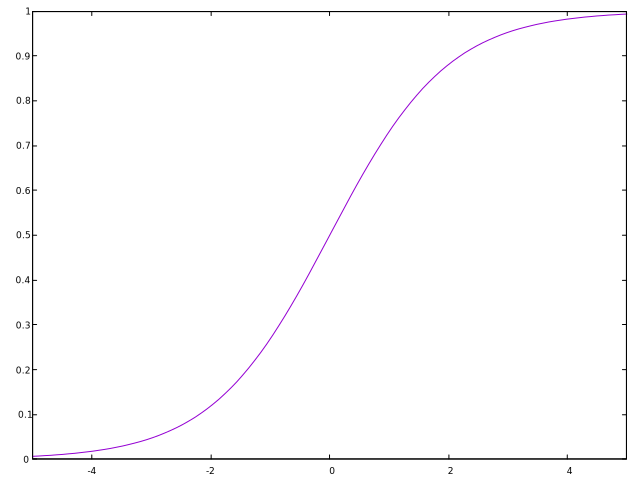
\includegraphics[width=0.5\linewidth]{sigmoid.png}
	\caption{sigmoid functie}
\end{figure}
Dit gebruiken zorgt ervoor dat de sigmoid neuron gelijkaardig is voor zeer grote en kleine waarden van $z \equiv w \cdot x + b$ aan de perceptron (respectievelijk wordt ze gemapt op ongeveer 1 en 0).\\
Er kan ingezien worden dat dit de 'smoothed' versie is van de stapfunctie
\begin{equation}
f(z) = \left\{
	\begin{tabular}{ccc}
		0 & als & $z \leq$ 0 \\
		1 & als & $z >$ 0 \\
	\end{tabular}
\right\}
\end{equation}
als $\sigma$ dit was bekwamen we een perceptron, door sigmoid te gebruiken hebben we nu een continue functie waardoor ons gevraagde, een kleine verandering aan de gewichten en bias $\to$ kleine verandering aan de output, wordt bekomen. Via calculus bekomen we dat:
\begin{equation}
	\Delta output \approx \sum_{j}\frac{\partial output}{\partial w_j}\Delta w_j + \frac{\partial output}{\partial b} \Delta b
\end{equation} 
Het is enkel de vorm van de functie die ertoe doet, het dient niet per se $\sigma$ te zijn. Ze is echter een goede beginfunctie om mee vertrouwd te geraken en wordt nog veel gebruikt (ook is het afleiden simpel), later zal nog met andere functies $f(\cdot)$ gewerkt worden.
Om achteraf te weten of iets effectief waar of niet waar is kan dan bv gekozen worden dat ze boven of onder 0.5 ligt.
\subsection{benaming}
\begin{figure}[H]
	\centering
	\includegraphics[width=0.5\linewidth]{benaming.png}
\end{figure}
De neuronen van de inputs heten de input neuronen en degenen aan de output de output neuronen. Het aantal neuronen in de hidden layers is niet zo simpel en er gaat heel wat bedenking en overwegingen aan te pas die we later zullen bespreken.\\
Hier beschouwen we geen loops in onze modellen, deze soort modellen bestaan wel en worden 'recurrent neural networks' genoemd maar we zullen hier niet naar kijken.
\newpage
\section{een simpel netwerk om handgeschreven cijfers te classificeren}
\begin{figure}[h!]
	\centering
	\includegraphics[width=0.5\linewidth]{netwerk}
	\caption{3-lagen neural network}
	\label{netwerk}
\end{figure}
Om een eenvoudig netwerk te bouwen om cijfers te classificeren gebruiken we een model als in figuur \ref{netwerk}, hierbij gebruiken we een 3 lagen netwerk, 784 input layers die greyscale waarden tussen 0 en 1 binnenkrijgen, aangezien we als trainingdata MNIST data set zullen gebruiken van UCI waarbij foto's van 28 bij 28 zijn (28x28 = 784), en voor de hidden layer zal geëxperimenteerd worden met de hoeveelheid neuronen, voor nu 15. Dit zou ook kunnen gedaan worden met 4 outputs ipv 10 door te werken met het binair getalsysteem, het blijkt echter dat ze dan trager en slechter leert. Dit kan logisch ingezien worden door te stellen dat het makkelijker is kenmerken van een bepaald cijfer te achterhalen dan een 'most significant bit'  (dit is echter puur uit het abstract met geen formele aantoning maar echter een bruikbare vorm van intuïtievorming).
\section{Leren met gradient descent}
Om te kwantificeren hoe goed  werkt voeren we de 'cost functie' in:
\begin{equation*}
\mathfrak{C} \equiv \frac{1}{2n}\sum_{x}^{}\Vert y(x)(input)-\mathbf{a}(output) \Vert ^2
\label{kostfunctie}
\end{equation*}
met n het aantal training inputs, $\vec{a}$ de vector van outputs van het netwerk als x de input is en y(x) wat de output a dient te zijn. Deze wordt ook wel de 'quadratische cost functie' genoemd of de 'mean squared error' MSE, deze is arbitrair gekozen maar lijkt goed te werken. Ons netwerk werkt dus zoals we willen als $\mathfrak{C} \approx 0$, we willen ze dus minimaliseren, we doen dit aan de hand van 'gradient descent', onze kost functie $\mathfrak{C}(x,y)$ kan er bijvoorbeeld als volgt uitzien (dit is een zeer eenvoudig voorbeeld waarbij het minimum met het blote oog kan gevonden worden maar dient puur als voorbeeld):
\begin{figure}[H]
	\centering
	\includegraphics[width=0.5\linewidth]{cost_function}
\end{figure}
Minimum vinden door extremum met calculus te achterhalen is een nachtmerrie als er veel variabelen opduiken, daarom gaan we naar een analoog van een bal die van een vallei rolt, we kunnen hiervoor een willekeurige positie van de bal nemen en het traject berekenen aan de hand van afgeleiden van $\mathfrak{C}$, deze zouden ons alles vertellen over de vorm van de vallei en dus waar de bal naartoe dient te gaan, we doen dit als volgt:\\
Stel we gaan een kleine hoeveelheid $\Delta \nu_1$ in de $\nu_1$ richting en een kleine hoeveelheid $\Delta \nu_2$ in de $\nu_2$ richting. De wiskunde vertelt ons dat $\mathfrak{C}$ als volgt zal veranderen:
\begin{equation}
	\Delta \mathfrak{C} \approx \frac{\partial \mathfrak{C}}{\partial \nu_1}\Delta \nu_1 + \frac{\partial \mathfrak{C}}{\partial \nu_2}\Delta \nu_2
\end{equation}
Nu willen we een manier vinden om $\Delta \nu_1$ en $\Delta \nu_2$ zo te kiezen dat $\Delta \mathfrak{C}$ negatief is en dus de bal naar beneden rolt. Hiervoor definiëren we voor het gemak $\mathbf{\Delta\nu} := (\Delta \nu_1,\Delta \nu_2)^T$ nu is de gradiëntvector van $\vec{\nabla}\mathfrak{C} \equiv (\frac{\partial \mathfrak{C}}{\partial \nu_1},\frac{\partial \mathfrak{C}}{\partial \nu_2})^T$ en dus
\begin{equation}
	\Delta \mathfrak{C} \approx \vec{\nabla} \mathfrak{C} \cdot \mathbf{\Delta \nu}
\end{equation}
Deze vergelijking laat ons inzien hoe we $\mathbf{\Delta \nu}$ kunnen kiezen om $\Delta \mathfrak{C}$ negatief te maken, stel dat we
\begin{equation}
	\mathbf{\Delta \nu} = -\eta \vec{\nabla}\mathfrak{C}
	\label{learning rate}
\end{equation}
kiezen met $\eta$ klein en positief (de \textcolor{blue}{learning rate}) dan is
\begin{equation}
	\Delta \mathfrak{C} \approx -\eta \vec{\nabla}\mathfrak{C}\cdot\vec{\nabla}\mathfrak{C} = -\eta \Vert \vec{\nabla}\mathfrak{C}\Vert^2
\end{equation}
wat kleiner dan of gelijk aan nul is aangezien $\Vert \vec{\nabla}\mathfrak{C}\Vert^2 \geq 0$, we gebruiken dan vergelijking \ref{learning rate} om $\mathbf{\Delta \nu}$ te berekenen en de bal met die hoeveelheid te bewegen:
\begin{equation*}
	\nu \rightarrow \nu ' = \nu - \eta \vec{\nabla} \mathfrak{C}
	\label{descent function}
\end{equation*}
Die we dan opnieuw en opnieuw kunnen doen tot we het minimum hebben gevonden, hierbij is de juiste keuze van $\eta$ cruciaal: als deze te groot is kan $\Delta \mathfrak{C} > 0$ wat we niet willen en een te kleine kan een te traag algoritme leveren. Het vorig besprokene gaat natuurlijk makkelijk over in hogere dimensies met meerdere variabelen, er wordt gezegd dat vergelijking \ref{descent function} de 'gradient descent' definieerd, deze regel werkt echter niet altijd en we zullen hier later op terug komen. We zullen een limiet leggen op de grootte van de bewegingen volgens: $\Vert \mathbf{\Delta \nu} \Vert = \sigma$ voor een kleine $\sigma > 0$. Het kan bewezen worden dat de keuze van $\mathbf{\Delta \nu}$ die $\vec{\nabla} \mathfrak{C} \cdot \mathbf{\Delta \nu}$ het snelst minimaliseert \ref{learning rate} is met $\eta = \frac{\sigma}{\Vert \mathfrak{C} \Vert}$ is (via Cauchy-Schwarz). Nu kan dit idee gebruikt worden om de gewichten $w_k$ en biasen $b_l$ te vinden die de kost functie minimaliseert, hierbij veranderen ze dus de variabelen $\nu_j$ oftewel onze 'positie'. Als we deze update regel hiervoor dus in componenten uitschrijven bekomen we:
\begin{equation*}
w_k \rightarrow w_k ' = w_k - \eta \frac{\partial \mathfrak{C}}{\partial w_k}
\end{equation*}
\begin{equation*}
b_l \rightarrow b_l ' = w_k - \eta \frac{\partial \mathfrak{C}}{\partial b_l}
\end{equation*}
Er treden veel moeilijkheden op hiervoor die we later zullen bespreken, nu bespreken we enkel 1 bepaald probleem:\\
Merk op dat de cost functie de vorm $\mathfrak{C} = \frac{1}{n}\sum_{x}\mathfrak{C}_x$ heeft, dus een gemiddelde over de costs $\mathfrak{C} \equiv \frac{\Vert y(x) -a \Vert ^2}{2}$ van individuele trainings. In de werkelijkheid om $\vec{\nabla}\mathfrak{C}$ te berekenen dienen we $\vec{\nabla}\mathfrak{C}_x$'s apart te berekenen voor elke input x en daar het gemiddelde van nemen, dit is echter zeer traag als het aantal training inputs zeer groot is.Daarom werken we met een systeem genaamd \textcolor{blue}{stochastic gradient} waarbij $\vec{\nabla}\mathfrak{C}$ geschat wordt door $\vec{\nabla}\mathfrak{C}_x$ te berekenen voor een kleine random sample en daar het gemiddelde van nemen en zo een goede benadering van $\vec{\nabla}\mathfrak{C}$ bekomen. Hiervoor kiezen we een kleine hoeveelheid m random inputs: $X_1,X_2,...,X_m$ die we een \textcolor{blue}{mini-batch} noemen, als deze groot genoeg is dan:
\begin{equation*}
	\frac{\sum_{j=1}^{m}\vec{\nabla} \mathfrak{C}_{X_j}}{m} \approx \frac{\sum_{x}^{}\vec{\nabla} \mathfrak{C}_{x}}{n} = \vec{\nabla} \mathfrak{C}
\end{equation*}
met de $2^{de}$ som over de volledige dataset, de zijden verwisselen geeft dus dat:
\begin{equation*}
	\vec{\nabla} \mathfrak{C} \approx \frac{1}{m}\sum_{j=1}^{m}\vec{\nabla} \mathfrak{C}_{X_j}
\end{equation*}
en dus werkt stochastic gradient descent door een random mini-batch te nemen en ermee als volgt te trainen:
\begin{equation}
w_k \rightarrow w_k ' = w_k - \frac{\eta}{m} \sum_{j}^{}\frac{\mathfrak{C}_{X_j}}{\partial w_k}
\label{stochastic_1}
\end{equation}
\begin{equation}
b_l \rightarrow b_l ' = b_l - \frac{\eta}{m} \sum_{j}^{}\frac{\mathfrak{C}_{X_j}}{\partial b_l}
\label{stochastic_2}
\end{equation}
Waar de sommaties over al de training examples $X_j$ zijn in de momentane mini-batch, hierna natuurlijk een andere random batch kiezen en daarmee trainen en zo verder tot ze zijn opgebruikt. We hebben dan een \textcolor{blue}{epoch} aan training voltooid. Hierna starten we met een nieuwe training epoch.\\
Let wel op dat de $\frac{1}{n}$ term in vergelijking \ref{kostfunctie} kan weggelaten worden om te sommeren over individuele trainings ipv uit te middelen, dit kan handig zijn als het aantal trainingdata niet vooraf bekend is. Ook wordt de $\frac{1}{m}$ term in vergelijking \ref{stochastic_1} en \ref{stochastic_2} vaak weggelaten, dit geeft geen verschil aangezien $\eta$ gewoon kan herschaald worden.\\
\subsection{Mathematische schrijfwijze}
Een gewicht gaande van de $k^{de}$ neuron in de $2^{de}$ laag naar de $j^{de}$ in de 3de laag noteren we met $w_{jk}$, het voordeel aan deze schrijfwijze is dat de vector van activaties van de $3^{de}$ laag dit geeft:
\begin{equation}
\sigma\left(
\begin{pmatrix}
w_{0,0} & w_{0,1} & \cdots & w_{0,k} \\
w_{1,0} & w_{1,1} & \cdots & w_{1,k} \\
\vdots  & \vdots  & \ddots & \vdots  \\
w_{j,0} & w_{j,1} & \cdots & w_{j,k} 
\end{pmatrix}
%
\begin{bmatrix}
a_0^{(1)} \\
a_1^{(1)} \\
\vdots \\
a_n^{(1)} \\
\end{bmatrix} 
%
+
\begin{bmatrix}
b_0\\
b_1\\
\vdots \\
b_n\\
\end{bmatrix} 
\right)
=
%
\begin{bmatrix}
a_0^{(2)} \\
a_1^{(2)} \\
\vdots \\
a_n^{(2)}\\
\end{bmatrix} 
\end{equation}
of kort
\begin{equation}
	\mathbf{a^{(2)}} = \sigma(\mathbf{Wa^{(1)} + b})
	\label{vergelijking_22}
\end{equation}
Waarbij de exponent de laag voorstelt (beginnende aan 0).

\section{Implementeren van ons netwerk om getallen te classificeren}
Wij zullen gebruik maken van 50000 van de 60000 foto's uit de data set om later dingen te kunnen uitspoken met de overige 10000.
Eerst en vooral zullen we een class \textit{Netwerk} maken die we zullen gebruiken om ons neural network voor te stellen:
\begin{minted}{python}
import numpy as np
class Netwerk(object):
	
 def __init__(self, groottes):
   self.aantal_lagen = len(groottes)
   self.groottes = groottes
   self.biases = [np.random.randn(y, 1) for y in groottes[1:]]
   self.gewichten = [np.random.randn(y, x)
               for x, y in zip(groottes[:-1], groottes[1:])]
\end{minted}
Hierbij bevat de lijst groottes het aantal neuronen in de respectievelijke lagen, een netwerk met 2 in de eerste, 3 in de $2^{de}$ en 1 in de laatste zou bijvoorbeeld gevormd worden met: \mint{python}{net=Netwerk([2, 3, 1])}
de biases en gewichten in het \textit{Netwerk} object zijn allemaal random via de Numpy np.random.randn functie die gaussische distributies genereert met gemiddelde 0 en standaarddeviatie 1, dit zorg dus voor een random plaats van waar het 'stochastic gradient descent' algoritme kan vertrekken. Later zullen we betere startmogelijkheden bespreken maar voorlopig is dit goed.
Hier is de code met wat extra uitleg maar probeer ze eerst zelf te ontcijferen:
\newpage
\mint{python}{self.biases = [np.random.randn(y, 1) for y in groottes[1:]]}
\vspace{0.2cm}
Dit maakt een lijst van arrays (hoeveelheid afhankelijk van hoeveel hidden lagen) waarbij
de arrays elk het aantal neuronen per laag bevatten aan items die elk gaussisch gegenereerde getallen
zijn. Het vorig voorbeeld geeft dan bijvoorbeeld [array([[ 0.67097482],[-0.07362273],[-1.05704179]]),
array([[-1.14542345]])]
\mint{python}{self.gewichten = [np.random.randn(y, x) for x, y in zip(groottes[:-1], groottes[1:])]}
\vspace{0.2cm}
De zip geeft een lijst terug van tuples die de overgangen voorstellen, met dit voorbeeld dus [(2,3),(3,1)].
np.random.randn(y,x) geeft een array van y vectoren terug van elk x elementen, bij dit voorbeeld dus
[array([[-0.5024744 , -0.26511926],
[ 0.6797002 , -0.79437011],
[ 0.00753035,  0.15947405]]),
array([[ 0.98995451, -1.17216928, -2.05475119]])].\\
Oftewel is per array een laag neuronen en die array bevat de gewichten per neuron die binnenkomen, dit kan voorgesteld worden in de vorm van een matrix, bijvoorbeeld heeft de $2^{de}$ laag als gewichten (0.98995451 , -1.17216928 , -2.05475119) $\equiv$ ($w_{0,0} , w_{0,1} , w_{0,2}$) oftewel de verbindingen tussen de 3 neuronen in de $2^{de}$- en de ene in de derde laag.\\
Nu dienen we nog de simoid functie te definiëren:
\begin{minted}{python}
def sigmoid(z):
  return 1.0/(1.0+np.exp(-z))
\end{minted}
Als de input z een vector of een Numpy array is wordt de functie automatisch per element toegepast (dit kan enkel met arrays, niet met lists). Nu dienen we nog een \textit{feedforward} methode te maken in de \textit{Netwerk}, dit neemt als input a en geeft de corresponderende output, dus gewoon vergelijking \ref{vergelijking_22} uitvoeren voor elke laag.

\begin{minted}{python}
def feedforward(self, a):
  for b, w in zip(self.biases, self.weights):
    a = sigmoid(np.dot(w, a)+b)
  return a
\end{minted}

Nu het effectieveve onderdeel implementeren waarmee ons \textit{Netwerk} gaat leren, een 'stochastic gradient descent' definitie \textit{SGD}:
\begin{minted}{python}
def SGD(self, training_data, epochs, mini_batch_size, eta,
test_data=None):

  if test_data: n_test = len(test_data)
  n = len(training_data)
  for j in xrange(epochs):
    random.shuffle(training_data)
    mini_batches = [
      training_data[k:k+mini_batch_size]
      for k in xrange(0, n, mini_batch_size)]
    for mini_batch in mini_batches:
      self.update_mini_batch(mini_batch, eta)
    if test_data:
      print "Epoch {0}: {1} / {2}".format(
      j, self.evaluate(test_data), n_test)
    else:
      print "Epoch {0} complete".format(j)
\end{minted}
Dit traint het neural network met mini-batch stochastic
gradient descent. "$training\_data$" Is een lijst van tuples
"(x, y)" die de training inputs en de gewenste
outputs voorstellen. als "$test\_data$" wordt gegeven dan zal het
netwerk geëvalueerd worden tegen de test data na elke
epoch, en wordt de geleidelijke vooruitgang geprint. Dit is bruikbaar om te zien hoe het vordert
maar vertraagd het process heel veel.
Nu zullen we kijken naar het updaten van de mini batch; de code ziet er als volgt uit:
\newpage
\begin{minted}{python}
def update_mini_batch(self, mini_batch, eta):
        """Update the network's weights and biases by applying
        gradient descent using backpropagation to a single mini batch.
        The "mini_batch" is a list of tuples "(x, y)", and "eta"
        is the learning rate."""
        nabla_b = [np.zeros(b.shape) for b in self.biases]
        """Update het network zijn gewichten en biases door het toepassen van
        gradient descent dmv backpropagatie naar een enkele mini batch.
        De mini batch is net als de "totale batch" een lijst tuples "(x, y)", 
	en "eta"
        is de "learning rate"."""
        nabla_b = [np.zeros(b.shape) for b in self.biases] 
	#shape geeft de dimensie van het array b
        nabla_w = [np.zeros(w.shape) for w in self.weights]
        for x, y in mini_batch:
            delta_nabla_b, delta_nabla_w = self.backprop(x, y)
            nabla_b = [nb+dnb for nb, dnb in zip(nabla_b, delta_nabla_b)]
            delta_nabla_b, delta_nabla_w = self.backprop(x, y) 
	    #dees functie komt nog lol
            nabla_b = [nb+dnb for nb, dnb in zip(nabla_b, delta_nabla_b)] 
	    #de accent versie (nabla b')
            nabla_w = [nw+dnw for nw, dnw in zip(nabla_w, delta_nabla_w)]
        self.weights = [w-(eta/len(mini_batch))*nw
                        for w, nw in zip(self.weights, nabla_w)]
\end{minted}
Nu moeten we de mnist data laden in de vorm van tuples, zoals ze hier gebruikt worden.
\newpage

\section{Google Crash Course}
De eerste 95 minuten aan les gaan over evidente dingen en dingen die we in de vorige sectie gezien hebben (zoals cost function, gradiant descent, learning rate,...). Het deel van TensorFlow gaat echter over de high-level API\footnote{application programming interface} tf.keras wat de TensorFlow variant is van het open-source Keras API. Het gebruik hiervan vereist een bepaalde kennis van numpy en pandas, aangezien ik redelijk vloeiend ben in numpy zal ik hier enkel de notes van pandas deponeren:
\subsecion{Pandas}
\begin{minted}{python}
import numpy as np
import pandas as pd

#genereer een 3X4 pandas DataFrame met kolommen Eleanor, Chidi, Tahani en Jason
data = np.random.randint(101, size=(3,4))
KolomNamen = ['Eleanor','Chidi','Tahani','Jason']
DataFrame = pd.DataFrame(data=data,columns=KolomNamen)

#print voll dataframe:
print(DataFrame)

#print waarde van 1ste rij van de Eleanor kolom:
print(DataFrame['Eleanor'].iloc[[1]])

#maak een 5de kolom Janet die de waarde heeft van Tahani+Jason:
DataFrame['Janet'] = DataFrame['Tahani'] + DataFrame['Jason']                                                  
\end{minted}

\subsecion{Linear regression with tf.keras}

Hierbij wordt geëxperimenteerd met de zogenaamde "hyperparameters" (i.e de "learning rate", het aantal epochs en de mini-batch grootte) om zo optimaal mogelijk een rechte te fitten aan een gegeven dataset. De code hiervoor wordt nog niet verwacht om begrepen te worden en wordt dus voor later gehouden. In deze cursus wordt met de squared loss ($L_2$ loss) gewerkt als verliesfunctie $(observatie - voorspelling(x))^2$, enkele goede technieken om te weten of je goede hyperparameters hebt gekozen zijn dan:
\begin{itemize}
	\item het verlies daalt gelijkmatig, eerst snel dan trager (zie figuur \ref{verliesfunctie})
	\item als de verliesfunctie niet convergeerd $\rightarrow$ meer epochs
	\item te traag dalende verliesfunctie $\rightarrow$ grotere learning rate (niet te groot anders geen convergentie)
	\item als de verliesfunctie veel varieërt (rondspringt) $\rightarrow$ lagere learning rate
	\item het verlagen van de learing rate + verhogen v/h aantal epochs/grootte mini-batcehs is vaak een goede combo
	\item de batchgrootte te klein maken kan ook voor problemen zorgen. Werk groot $\rightarrow$ klein tot ze raar doet
	\item Soms is de dataset zo groot dat ze ni in uw ram past, hou daar rekening mee en neem een geschikte mini-batch
\end{itemize}
\begin{figure}
    \centering
    \begin{minipage}{0.45\textwidth}
        \centering
        \includegraphics[width=0.9\textwidth]{LinearRegression.png}
        \caption{Lineaire regressie}
    \end{minipage}\hfill
    \begin{minipage}{0.45\textwidth}
        \centering
        \includegraphics[width=0.9\textwidth]{LinearRegressionCost.png}
	\caption{verliesfunctie}
	\label{verliesfunctie}
    \end{minipage}
\end{figure}
Een echte dataset komt vaak in .csv (comma seperated values) formaat, dewelke er als volgt uit zien:
\\\\
\begin{table}[]
\begin{tabular}{lllllll}
longitude   & latitude  & housing\_median\_age & total\_rooms & population  & median\_income & median\_house\_value \\
\hline
\\
-114.310000 & 34.190000 & 15.000000            & 5612.000000  & 1015.000000 & 1.493600       & 66900.000000         \\
-114.470000 & 34.400000 & 19.000000            & 7650.000000  & 1129.000000 & 1.820000       & 80100.000000         \\
-114.560000 & 33.690000 & 17.000000            & 720.000000   & 333.000000  & 1.650900       & 85700.000000         \\
-114.570000 & 33.640000 & 14.000000            & 1501.000000  & 515.000000  & 3.191700       & 73400.000000        
\end{tabular}
\end{table}
\\\\
Uit "Linear regression with a real dataset" leren we deze csv openen met pandas en dat je moet oppassen met het gebruik van data  met rare waarden (bv. gemiddelde van 2600, met 25,50 en 75 percentiel onder 3100 maar wel een maximum van 38000). Nu kunnen we statistiek gebruiken om te kijken welke data corelleert met ons label. Een correlatiematrix indiceert hoeveel 2 datawaardes met elkaar gemeen hebben met als betekenis:
\begin{itemize}
	\item 1.0 perfecte correlatie (data 1 stijgt $\rightarrow$ data 2 stijgt)
	\item -1 perfecte negatieve correlatie (data 1 stijgt $\rightarrow$ data 2 daalt)
	\item 0.0 geen correlatie (niet lineair gerelateerd)
\end{itemize}
Zo'n matrix kan gemakkelijk met pandas worden gegenereerd, hebben we bv een csv bestand ingeladen:
\begin{minted}{python}
training_df = pd.read_csv(filepath_or_buffer=
  "https://download.mlcc.google.com/mledu-datasets/california_housing_train.csv")	
\end{minted}
Dan vinden we de correlatiematrix mbv
\begin{minted}{python}
	training_df.corr()
\end{minted}
Als we een model opbouwen moeten we 'overfitting' in acht nemen. Dit is het fenomeen waarbij, als we het model complexer maken dan nodig, de fout zeer laag ligt bij de training data maar dat bij testdata ze zeer slecht scoort. We dienen hierom maken dat de data zo simpel mogelijk wordt 'gefit'. Een manier om dit te testen is om de data in een {\bf training set} en een {\bf test set} te verdelen.De volgende 3 basisaannames zorgen tot algemeenheid:
\begin{itemize}
\item We nemen voorbeelden onafhankelijk en gelijk {\bf(independently and identically 'i.i.d')} at random uit de verdeling. m.a.w, voorbeelden hebben geen invloed op elkaar. In de echte wereld willen we dit bij uitzonderlijke gevallen niet (als bijvoorbeeld welke reclame te tonen aan iemand).
\item De verdeling is stationair {(\bf stationary)}, i.e de distributie verandert niet binnen de dataset. Dit is niet het geval bij bijvoorbeeld seizoensshoppen. 
	\item We nemen voorbeelden uit partities van eenzelfde distributie
\end{itemize}

\newpage
\bibliography{bronnen}
\bibliographystyle{plain}
\end{document}
